\documentclass{article}
\usepackage{graphicx}
\usepackage[round]{natbib}
\usepackage{float}
\usepackage{fullpage}

\renewcommand{\thefigure}{S\arabic{figure}}

\begin{document}
\title{Supplementary information for \texttt{phyx} (Phylogenetic tools for Unix)}

\author{Joseph W. Brown$^{\dagger}$, Joseph F. Walker$^{\dagger}$, and Stephen A. Smith\\\\
\normalsize{Department of Ecology \& Evolutionary Biology}\\
\normalsize{University of Michigan, Ann Arbor, MI 48109, USA}\\
\normalsize{$^{\dagger}$Equal contribution}}
% address is not supported by article class?!? the above is hacky workaround
%\address{Department of Ecology \& Evolutionary Biology, University of Michigan, Ann Arbor, MI 48109, USA}
%\date{\today}
\date{} % no date
\maketitle

\section{Example pipeline}
As described above, \texttt{phyx} uses a stream-centric approach to input and output that allows for programs to be linked together without the use of intermediate files. Here, we illustrate how four \texttt{phyx} programs can be linked via piping
and a simple shell loop to perform a full analytical pipeline:
\begin{enumerate}
\item Clean alignments individually using a Unix for loop (\texttt{pxclsq}).
\item Concatenate cleaned alignments into a supermatrix (\texttt{pxcat}).
\item Infer a ML tree (\texttt{RAxML} \citep{Stamatakis2014}).
\item Re-root the tree on the outgroups (\texttt{pxrr}).
\item Remove the outgroups (\texttt{pxrmt}).
\end{enumerate}
which would take the form:

\begin{verbatim}
for x in *.fa; do pxclsq -s $x -p 1.0 -o $x.phyx; done &&
pxcat -s *.phyx -o out.concat -p models && raxml -T 2
-m GTRCAT -p 12345 -q models -s out.concat -n RAxMLout
&& pxrr -g s1,s2 -t RAxML_bestTree.RAxMLout | pxrmt
-n s1,s2 -o trimmed.tre
\end{verbatim}

\section{Performance}
We briefly describe below the performance (speed) of some \texttt{phyx} programs relative to other existing tools.

\subsection{Sequence cleaning}
Cleaning sequences to ensure a certain level of matrix occupancy has become common place in many phylogenomic pipelines \citep{Dunn2013,YangSmith2014}. Here we compare two programs \texttt{Gblocks v0.91b} \citep{Gblocks} and \texttt{phyutility v2.2.6} \citep{SmithDunn2008} to the sequence cleaning procedure of \texttt{phyx} (\texttt{pxclsq}). The file sizes ranged from 10 sequences (234 kB) to 100,000 sequences (2.3 GB), with each sequence being 23,950 base pairs in length (Figure~\ref{fig:S1}). The implementation for sequence cleaning in \texttt{pxclsq} is highly similar to \texttt{phyutility}, in that it focuses on column occupancy (proportion of missing data) as a means of determining whether a sequence region should be cleaned (that is, removed). However, the two programs differ in one key respect: for amino acids \texttt{pxclsq} treats the ambiguous character ``X'' as missing data, whereas \texttt{phyutility} does not; we therefore restricted analyses to DNA to avoid this inconsistency. Additionally, although \texttt{Gblocks} implements a more sophisticated range of methods for cleaning sequences, we restricted (using the \texttt{-b1} argument) cleaning to focus solely on column occupancy to make timings directly comparable. All programs were instructed to remove sites if they contained greater than 60\% missing data. We found that \texttt{phyx} outperformed both \texttt{Gblocks} and \texttt{phyutility} for all dataset sizes and for the largest dataset \texttt{phyutility} was not able to clean the dataset due to a memory allocation error. The test was conducted on a laptop  containing 4 processors and 16 GB of memory, with 14 GB of that memory being allocated for \texttt{phyutility}.

\begin{figure}[H]
    \centering
    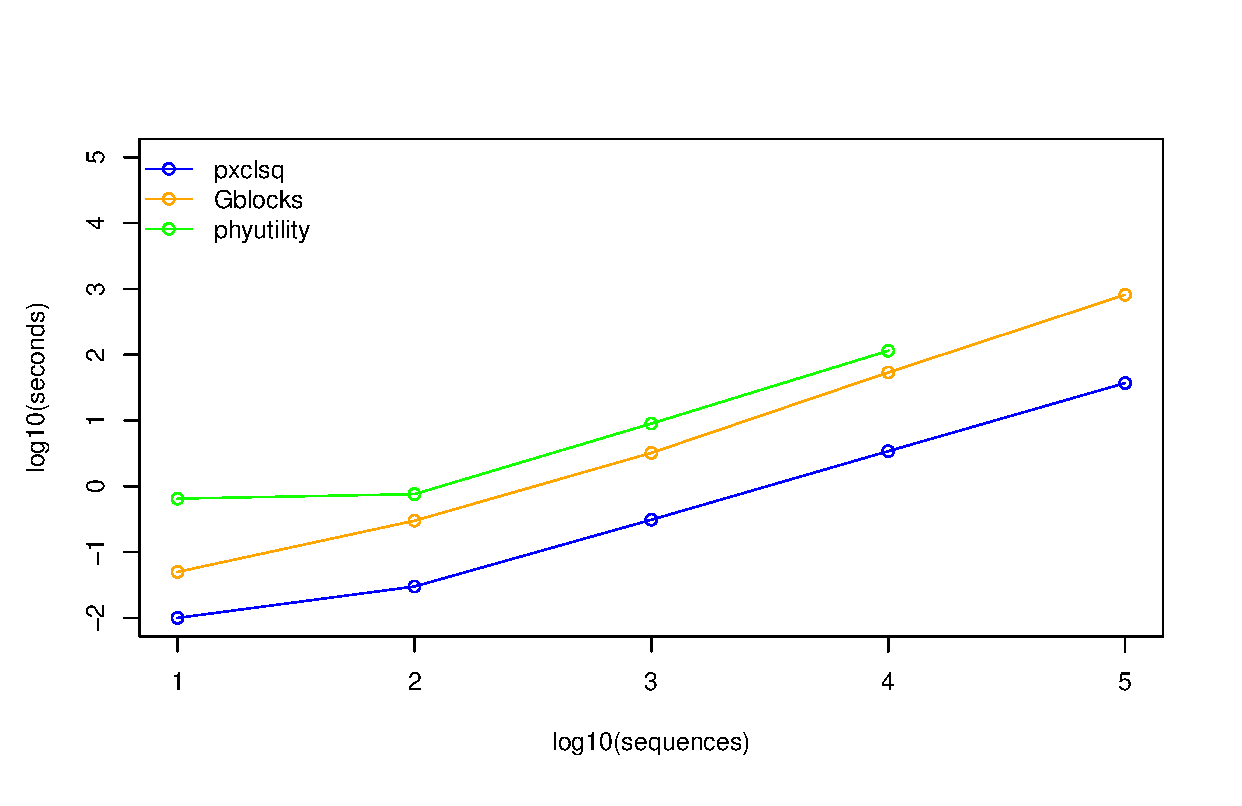
\includegraphics[width=5.0in]{clsq.eps}
    \caption{Comparison of alignment cleaning timings.}
    \label{cleaningfigure}
\label{fig:S1}
\end{figure}

\subsection{Conversion of proteins to codons}
Constructing a codon alignment from a protein alignment and its associated nucleotide matrix is necessary for both proper phylogenetic modelling (partitioning) and conducting positive selection tests. Here we tested the processing efficiency of files consisting of 801 amino acid residue sequences for between 10 and 10,000 taxa (file sizes ranging from 8 kB to 77 MB). We found that \texttt{phyx} program \texttt{aa2cdn} was faster than \texttt{PAL2NAL v14} \citep{Suyama2006} for all alignment sizes (Figure~\ref{fig:S2}). Importantly, unlike \texttt{PAL2NAL}, \texttt{aa2cdn} does not require that the sequences be in the same order across files, thus avoiding the possiblility of aligning a nucleotide sequence with something other than its corresponding amino acid sequence.

\begin{figure}[h]
    \centering
    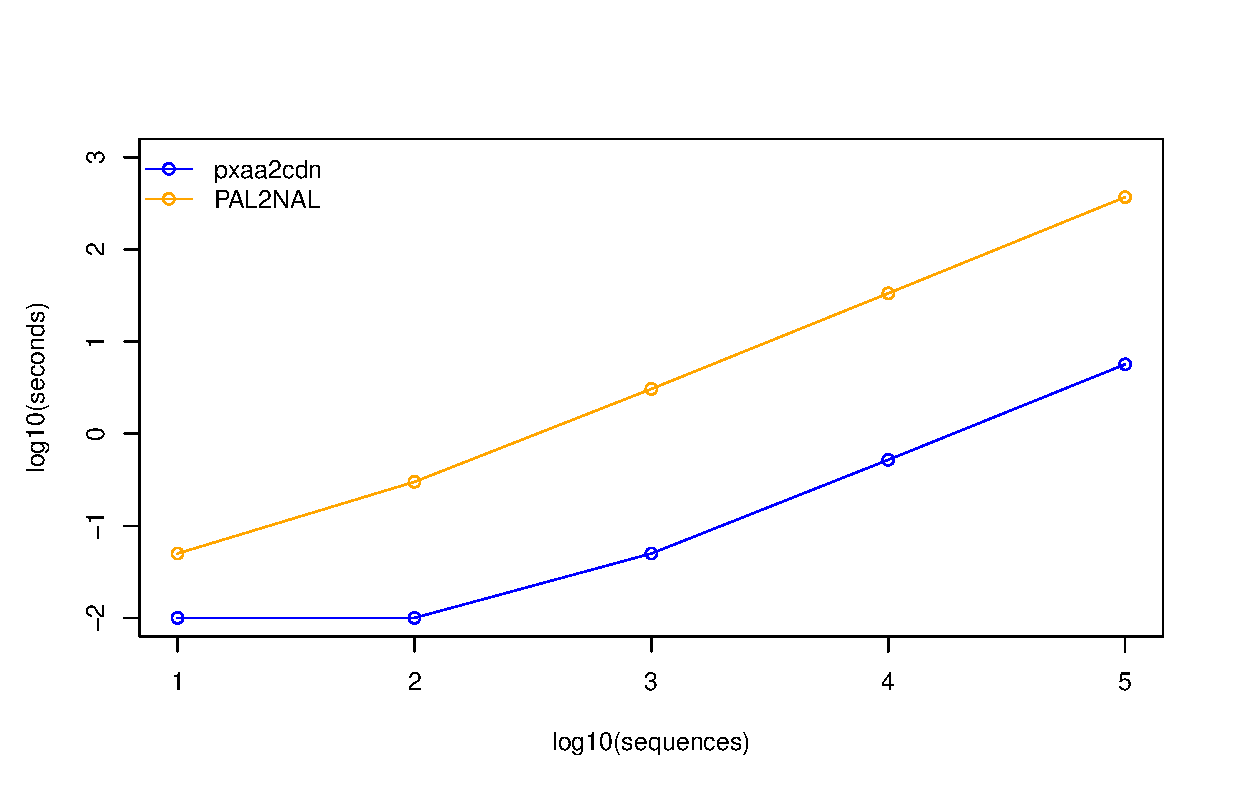
\includegraphics[width=5.0in]{aa2cdn}
    \caption{Comparison of timings to convert protein alignments to
    their corresponding codon alignments.}
    \label{proteincodonfigure}
\label{fig:S2}
\end{figure}

\subsection{MCMC log concatenation and resampling}
MCMC log files from Bayesian phylogenetic analyses have become common phylogenetic objects. Such analyses are typically replicated (to ensure convergence of the MCMC chains) and run for many millions of generations (to achieve adequate effective sample sizes), resulting in several very large text files, each of which invariably involve a burnin phase (samples that are discarded before sumamrization). Prior to parameter summary, these log files are typically concatenated while removing the burnin phase and potentially resampling (thinning) the individual logs because of memory constraints. The \texttt{phyx} program \texttt{pxlog} carries out these operations on both tree and parameter logs. To assess the performance of \texttt{pxlog}, we compared it to two versions of \texttt{logcombiner} from the \texttt{BEAST} package \citep{DrummondRambaut2007,Bouckaert2014}. We ran phylogenetic in analyses in \texttt{BEAST} using the data from \cite{Magallon2015}, a data set which consists of 798 taxa. Five replicate MCMC analyses were performed, each running for 100 million generations and sampling trees every 5000 generations (for a total of 20000 trees sampled in each analysis). In preparation for tree summary, we discarded the first 25\% of samples, and further thinned the chains to every 10th sample (for a total of 1500 post-burnin samples per analysis).

\begin{figure}[!h]
    \centering
    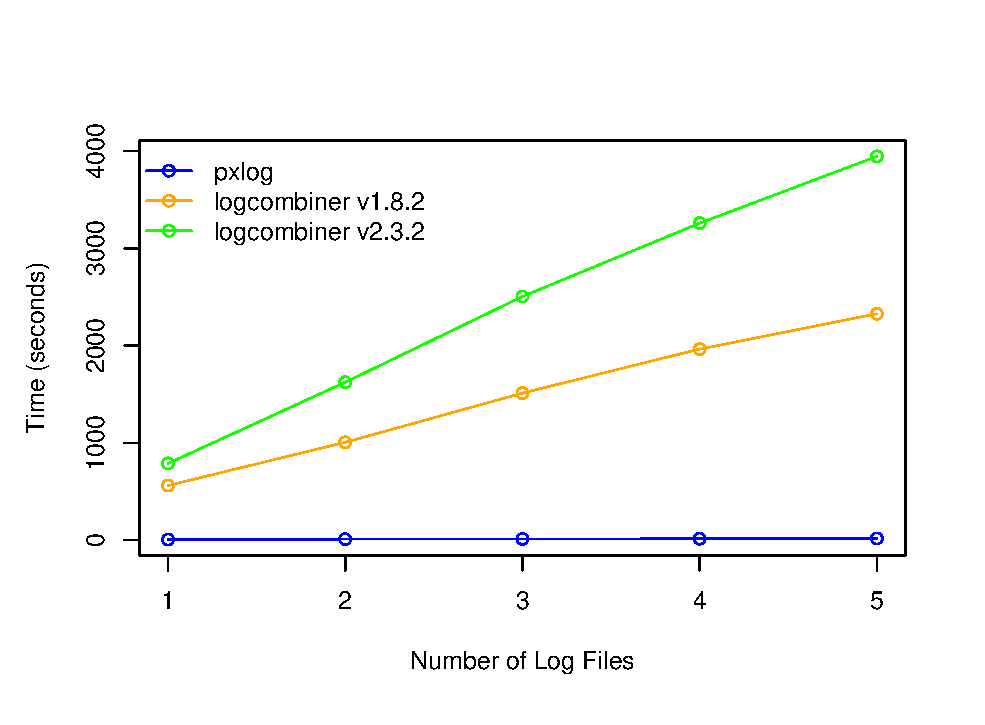
\includegraphics[width=5.0in]{log}
    \caption{Comparison of MCMC log manipulation timings. Each log file
    is 2.6 GB and contains 20000 trees.}
    \label{logfigure}
\label{fig:S3}
\end{figure}

The timings for the log manipulations by the various programs are displayed in Figure~\ref{fig:S3}. \texttt{pxlog} executed much faster than either version of \texttt{logcombiner} for any number of input files, taking only a few seconds compared to up to over an hour for the alternative tools. More revealing, however, was the memory usage of the various programs. \texttt{pxlog}, being stream-centric (and hence holding only a single tree in memory at any particular instant), consumed only 600 kb of RAM, despite the individual log files totalling 2.6 GB. \texttt{logcombiner} is a java-based tool to which we allocated 40 GB of RAM. \texttt{logcombiner v1.8.2} was far more memory efficient than the newer version, consuming 2.4 GB of RAM for the full 5 file concatenation. \texttt{logcombiner v2.3.2}, on the other hand, consumed 32.6 GB of RAM while executing far more slowly.

\bibliographystyle{natbib} % want this one, but acting wonky
%\bibliographystyle{abbrv}
%\bibliographystyle{achemnat}
%\bibliographystyle{plainnat}
%\bibliographystyle{abbrv}
%\bibliographystyle{bioinformatics}
%
%\bibliographystyle{plain}
\bibliography{phyx}

\end{document}
